\section{Технологическая часть}
В данной части рассматривается выбор средств реализации, описывается структура классов программы и приводится интерфейс программного обеспечения.

\subsection{Средства реализации}

Для написания данной курсовой работы был выбран язык C++~\cite{cpp-lang}.
Выбор данного языка программирования обусловлен следующим образом:
\begin{itemize}
	\item C++ --- объектно-ориентированный язык, а именно такая методология
	программирования была выбрана для разработки программы;
	\item в данном языке имеется большое количество библиотек и шаблонов,
	позволяющих не тратить время на изобретение готовых конструкций.;
	\item обладает высокими показателями вычислительной производительности, а так как требуется быстродействие задач генерации реалистичных изображений, то язык C++ необходим.
\end{itemize}

В качестве среды разработки был использован Qt Creator~\cite{qt-creator}.
Данный выбор обусловлен следующими факторами:
\begin{itemize}
	\item в QT Creator есть возможность быстрого создания интерфейса с помощью расширения QT Design;
	\item QT Creator обладает всем необходимым функционалом для написания, профилирования и отладки программ.
\end{itemize}

\subsection{Описание структуры программы}

На рисунке~\ref{fig:struct} представлена схема разработанных классов.

\begin{figure}[h]
	\centering
	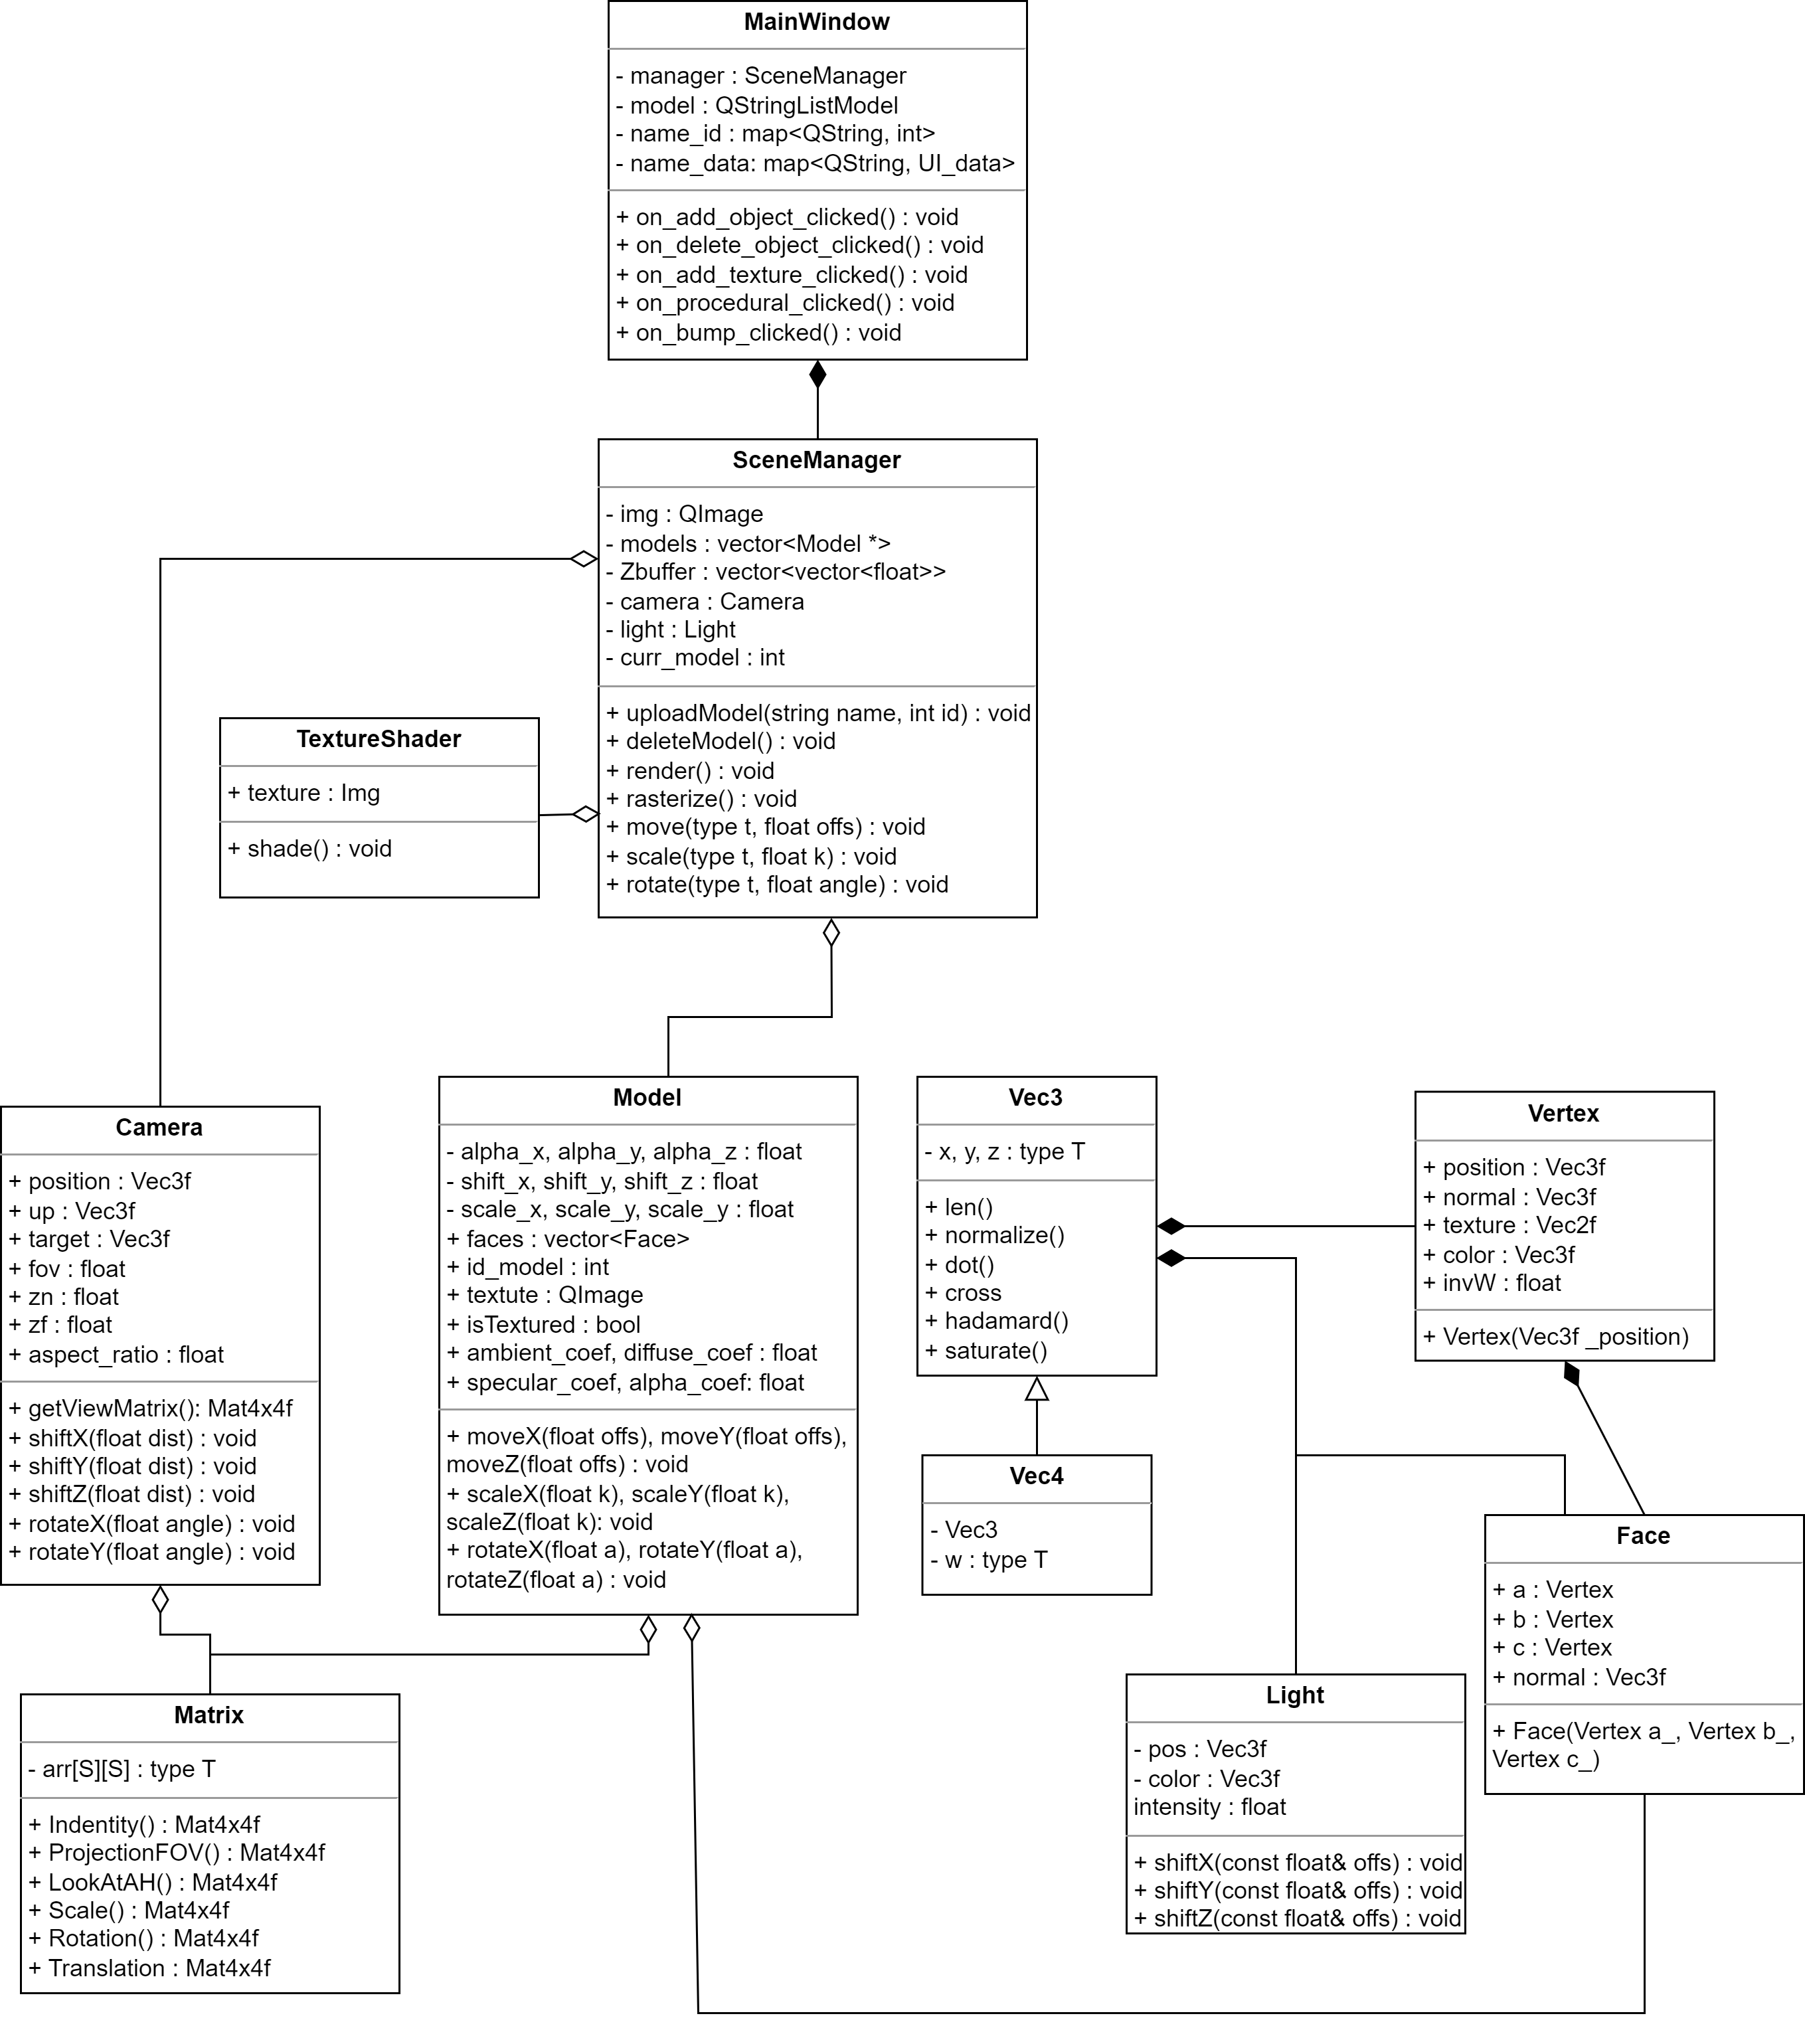
\includegraphics[width=0.9\textwidth]{img/algorithms/struct.png}
	\caption{Схема классов программы}
	\label{fig:struct}
\end{figure}
\clearpage
В программе реализованы следующие классы:
\begin{itemize}
	\item class SceneManager --- хранит сцену, описывает методы взаимодействия со сценой и объектами на ней;
	\item class Model --- описывает представление трёхмерного объекта и методы работы с ним;
	\item class Light --- описывает источники света и методы взаимодействия с ним;
	\item class Camera --- описывает камеру и методы взаимодействия с ней;
	\item class Vector --- реализация векторов размерности 3 и 4;
	\item class Matrix --- описывает матрицы и методы взаимодействия с ними.
	\item class TextureShader --- содержит функции для интерполяции значения текстурных координат в конкретном пикселе;
\end{itemize}

\subsection*{Вывод}
Было приведено описание структура программы, выбраны средства реализации программного обеспечения, приведены листинги кода, продемонстрирован интерфейс программы и представлены результаты работы программы. 
